% !TeX root = ../main.tex
% !TEX root = ../main.tex
% -*- root: ../main.tex -*-
% -*- program: pdflatex -*-
\chapter{构造公式方法}
上一章主要从插值方法入手介绍了对~TOF~的~MRPC~的离线数据的刻度方法。这一章将从构造公式入手对刻度进行研究。仍然采用击中位置和过阈时间分开修正的方法。其中对于击中位置的修正采用简单的多项式构造,对于过阈时间的修正,通过分析时间对过阈时间的分布,构造出几种简单的公式,并比较拟合的情况和拟合的结果,最终确定过阈时间项的公式。

\begin{figure}[!h]
\begin{minipage}[!h]{0.5\linewidth}
%\centering
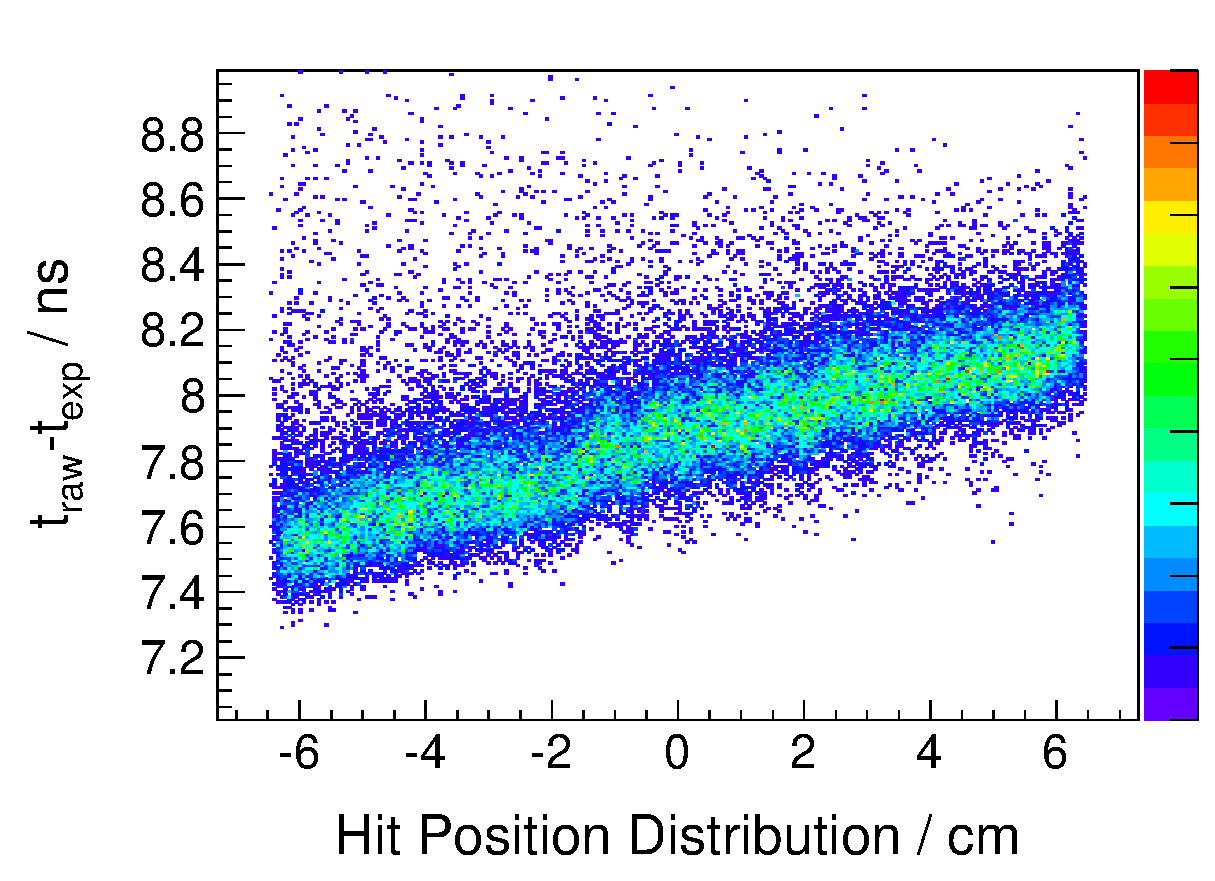
\includegraphics[width=0.9\textwidth]{chap3/left-tVSz.eps}
\subcaption{时间对击中位置的分布}
\label{fig:left-tVSz}
\end{minipage}%
\hfill
\begin{minipage}[!h]{0.5\linewidth}
%\centering
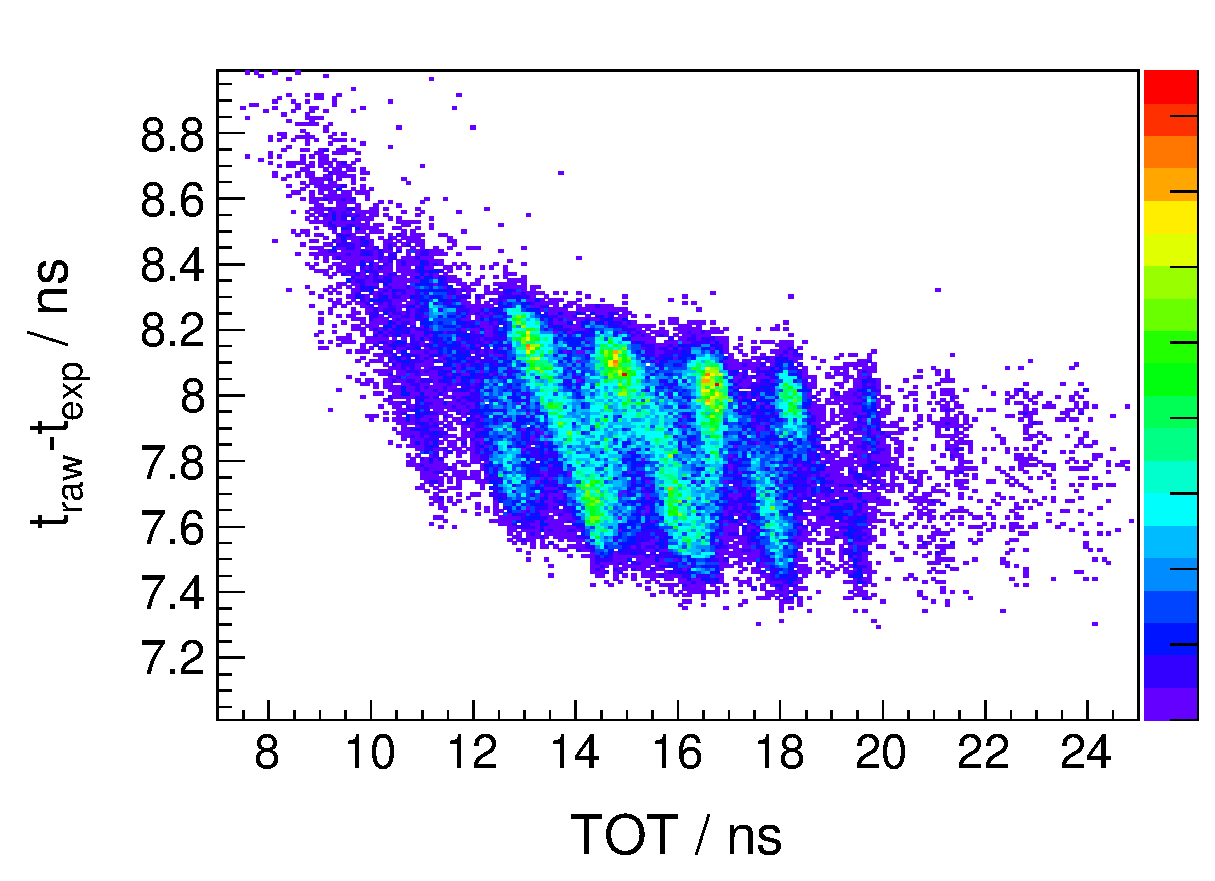
\includegraphics[width=0.9\textwidth]{chap3/left-tVSq.eps}
\subcaption{时间对~TOT~的分布}
\label{fig:left-tVSq}
\end{minipage}
\caption{时间对击中位置和过阈时间的分布}
\end{figure}

\section{击中位置的修正}
刻度修正的主要项之一就是击中位置项的修正。图~\ref{fig:left-tVSz}~时间与击中位置项的分布关系相对简单,几乎是线性关系,这一项主要是信号在对数条内的传播时间。图~\ref{fig:left-tVSz}~中的斜率表示的信号在读数条传播的有效速度。
\subsection{击中位置等区间分~bin~}

\begin{figure}[htbp]
\centering
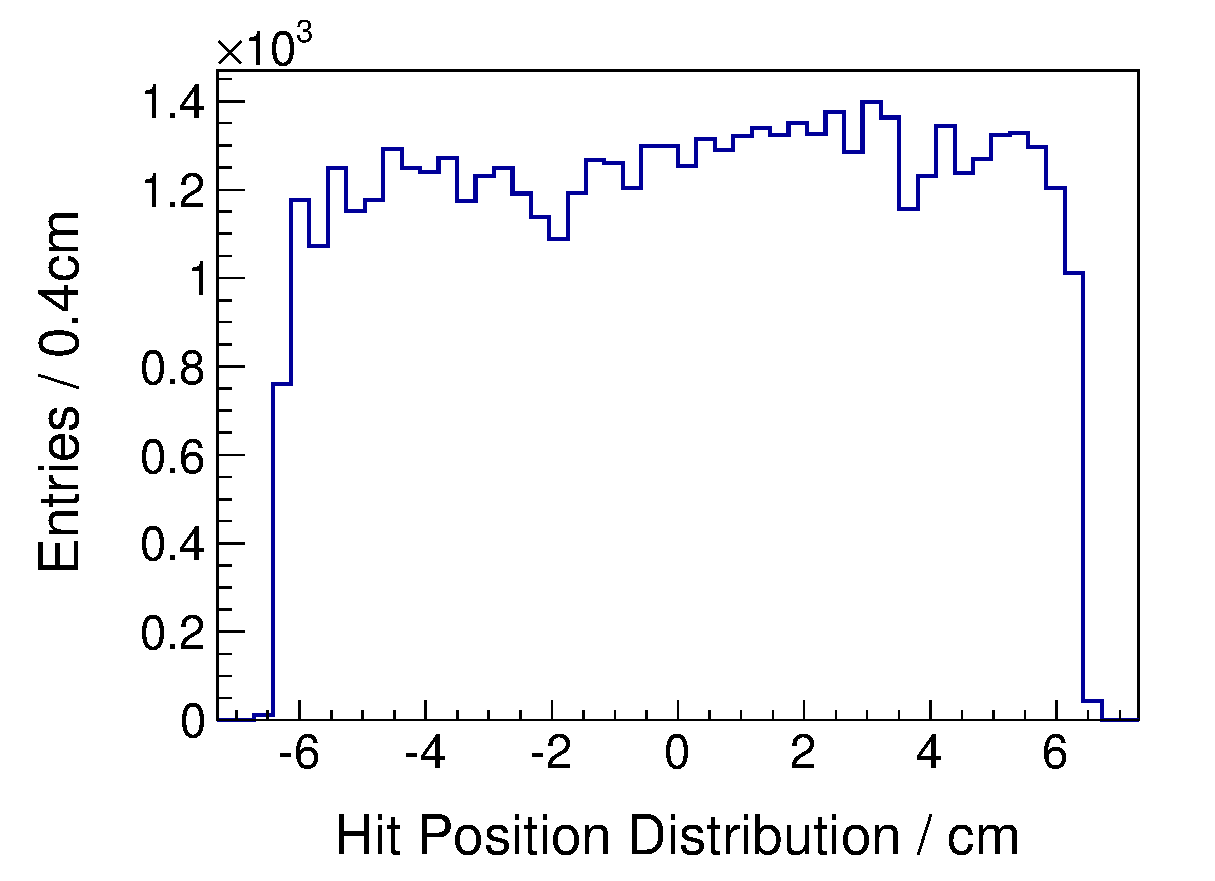
\includegraphics[width=0.5\textwidth]{chap3/left-z.eps}
\caption{击中位置的分布}
\label{fig:left-z}
\end{figure}

图~\ref{fig:left-z}~是击中位置的分布。可以看出,在此方向上事例数是均匀分布的,因此对击中位置的分~bin~采用等区间分~bin~方式。

图~\ref{fig:13bin}~是单个~bin~的时间分布。可以看出,这个分布左右并不完全对称,故不适合采用高斯拟合。考虑过采用朗道卷积一个高斯的拟合,但拟合的也并不十分贴切。

\begin{figure}[htbp]
\centering
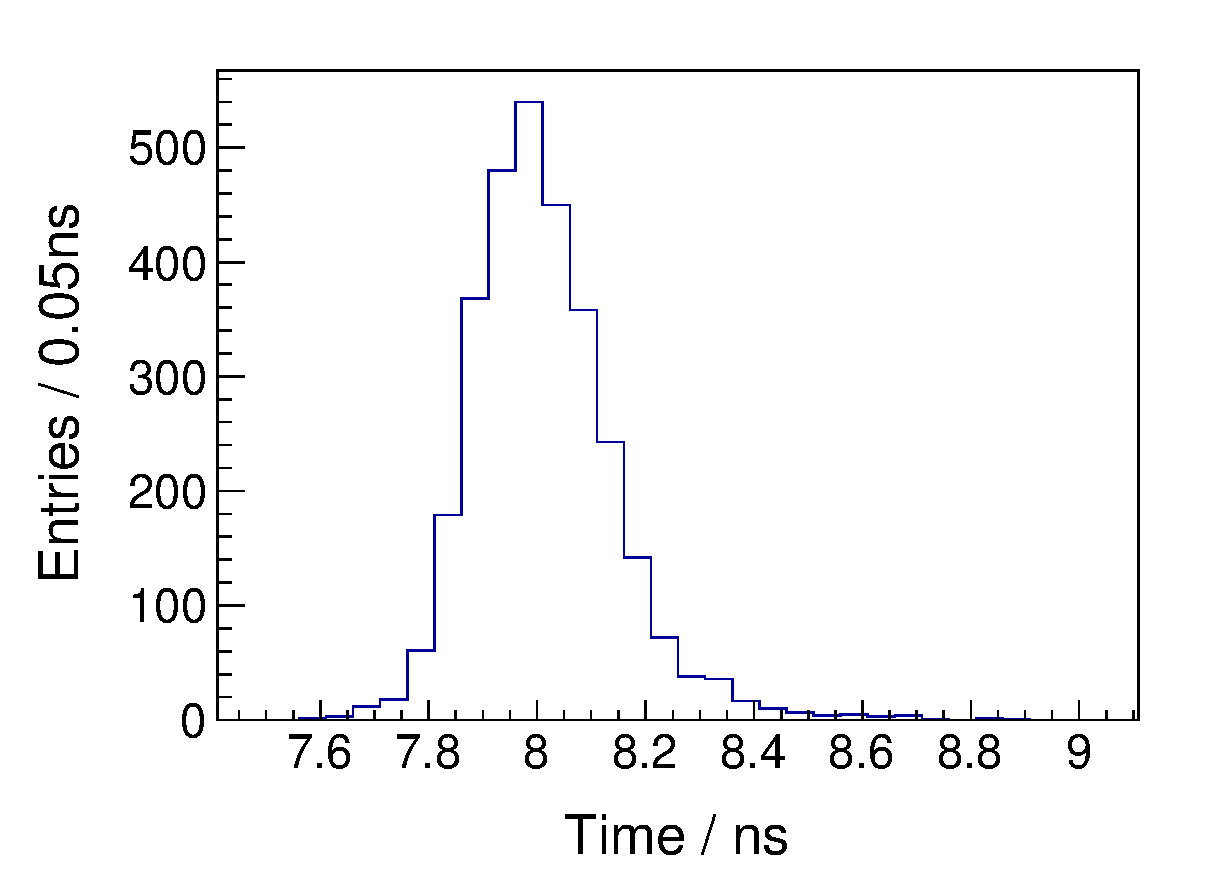
\includegraphics[width=0.5\textwidth]{chap3/13bin.eps}
\caption{单个~bin~的时间分布}
\label{fig:13bin}
\end{figure}

\subsection{每个~bin~采用~Nov~公式拟合}

从之前边渐鸣文章~Abosolute photon energy calibration for the BESIII EMC~ \cite{Bian:2010aa}~中看到关于${e^{+}e^{-} \to \gamma \gamma}$的分布也是左右不对称的,拟合采用的是一个~Novosibirsk\cite{Nov:2000aa}~的公式。
关于这个公式:
\begin{displaymath}
f_{Nov}(m)=Aexp(\frac{-ln^2(1+t\frac{sinh(t\sqrt{ln4})}{t\sqrt{ln4}}\frac{m-m_{0}}{\sigma})}{2t^2}-\frac{t^2}{2}) 
\end{displaymath}


~A~表示归一化常数,~$\sigma$~
表示时间分辨,~$m_{0}$~表示中心值,~$t(<0)$~表示参数化的尾巴。这个函数可以被看做是有一个不对称的尾巴的高斯函数。分析发现,这个函数形式对于拟合图~\ref{fig:13bin}~很合适。

\begin{figure}[htbp]
\centering
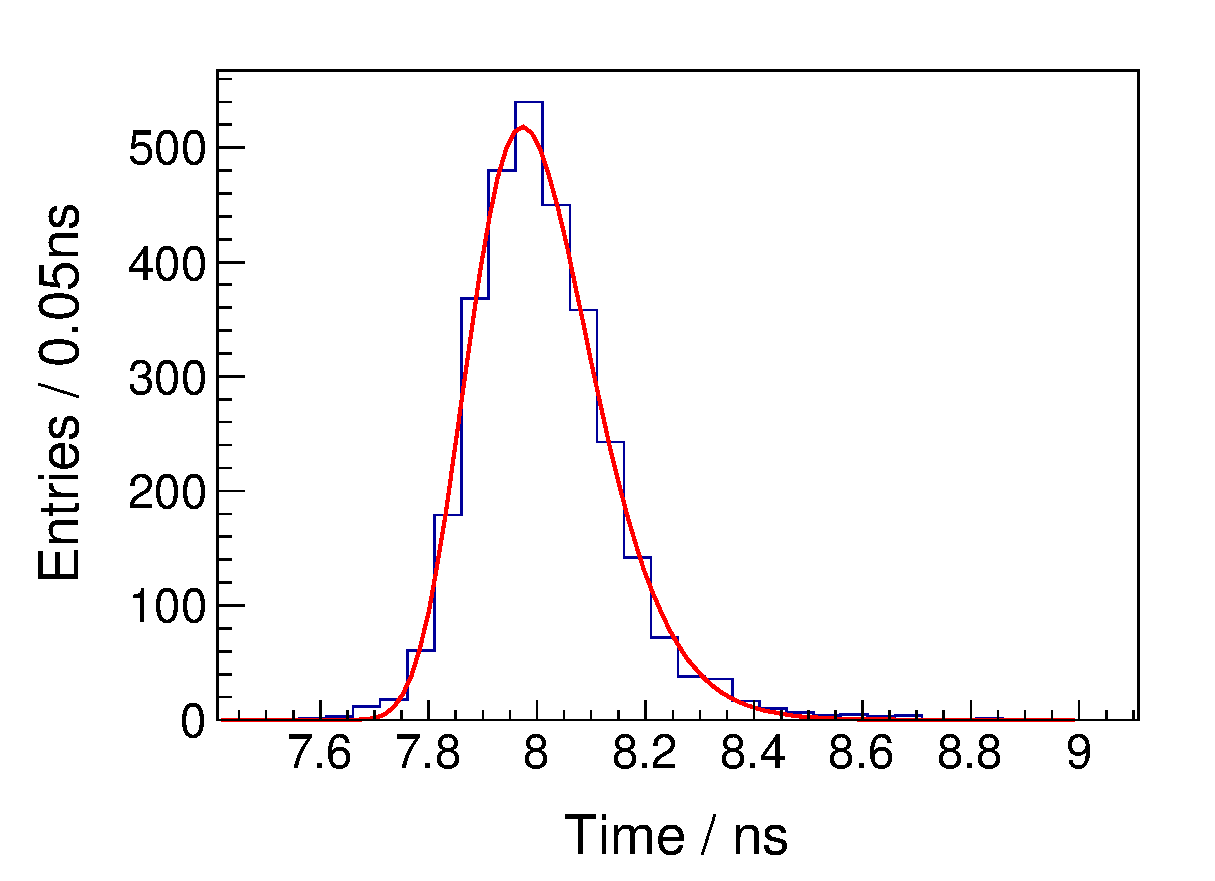
\includegraphics[width=0.5\textwidth]{chap3/13BinDraw.eps}
\caption{单个~bin~的时间用~Nov~公式拟合的结果}
\label{fig:13BinDraw}
\end{figure}

图~\ref{fig:13BinDraw}~是单个~bin~采用~Nov~公式拟合的结果。可以看出拟合的很好。

\begin{figure}[htbp]
\centering
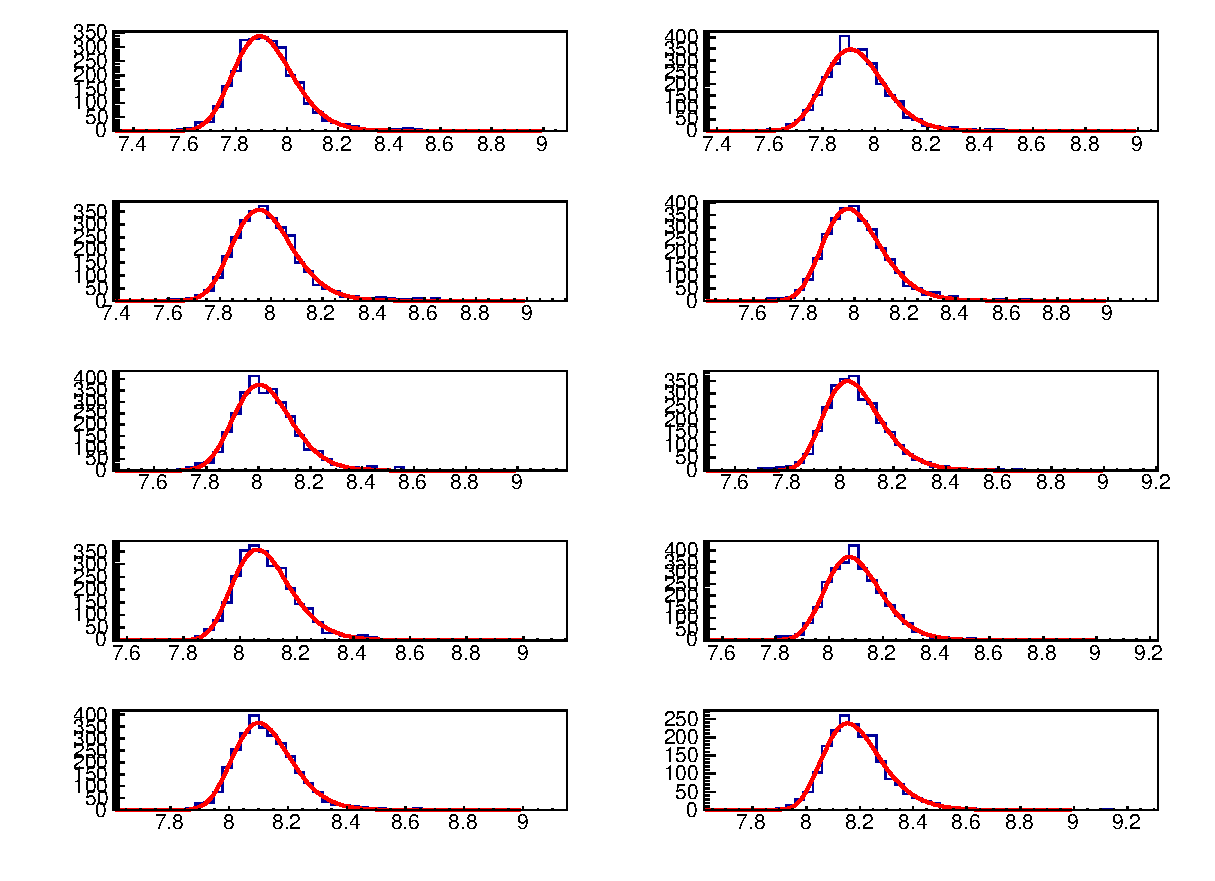
\includegraphics[width=0.85\textwidth]{chap3/10geDraw.eps}
\caption{10~个~bin~的时间用~Nov~公式拟合的结果}
\label{fig:10geDraw}
\end{figure}
图~\ref{fig:10geDraw}~是利用~Nov~公式对~10~个~bin~拟合情况,拟合的效果都比较好。所以对于击中位置分~bin~后就采用~Novsibirsk~公式进行拟合。

\subsection{对得到的~graph~点采用三阶多项式拟合}
上一小节研究得到了分~bin~后的每个~bin~的中心值。中心值拟合得到的曲线的斜率是等于信号在读数条内传播的有效速度,对此采用一个多项式拟合。如图~\ref{fig:z-fit}~

\begin{figure}[htbp]
\centering
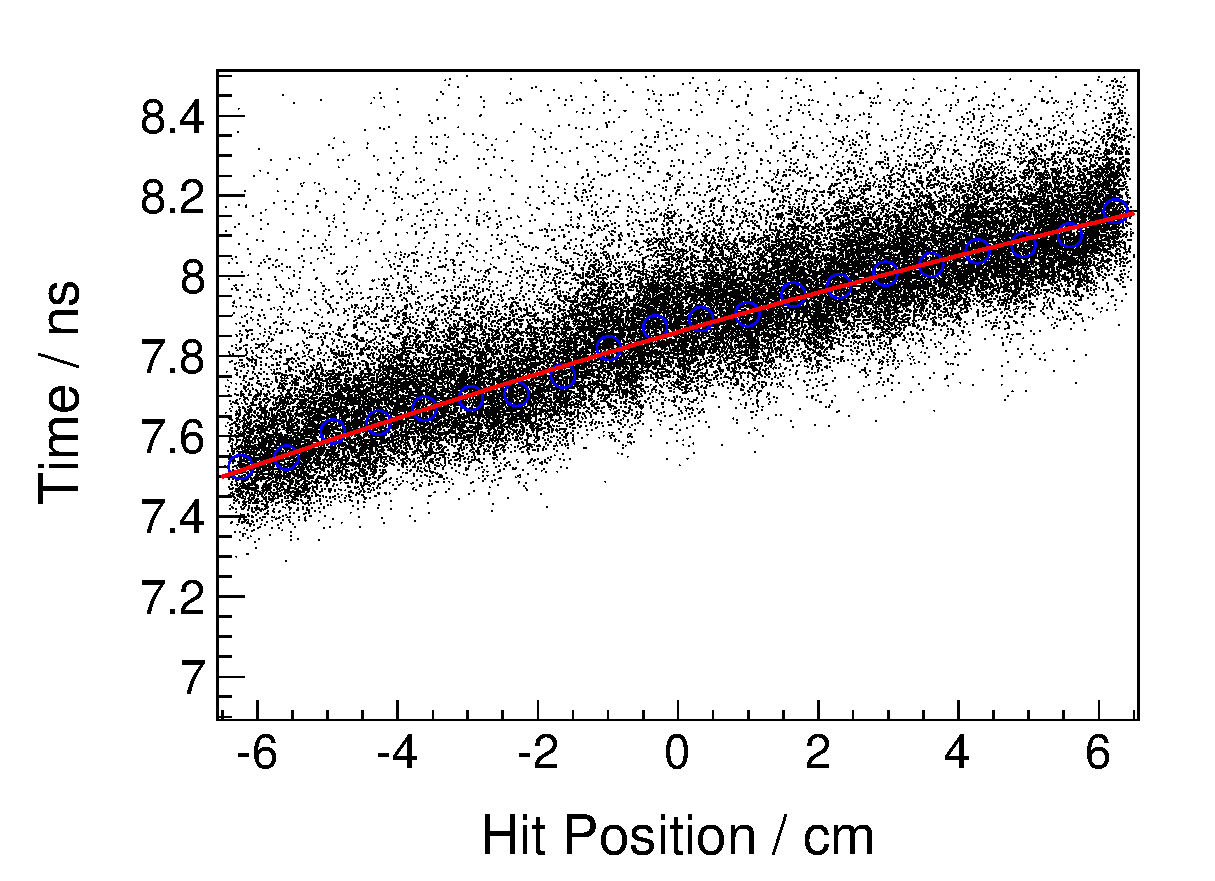
\includegraphics[width=0.9\textwidth]{chap3/z-fit.eps}
\caption{对击中位置采用多项式拟合}
\label{fig:z-fit}
\end{figure}
%这里选用的三阶多项式拟合。可以拟合出时间随击中位置的变化趋势。
\section{过阈时间的修正}
修正完击中位置的贡献后,时间与过阈时间的分布变得简单。
图~\ref{fig:afterCorZ-TOT}~是利用上述方法修正完击中位置后的时间对过阈时间的分布,此时时间对过阈时间的分布的折线现象基本消失。

\begin{figure}[htbp]
\centering
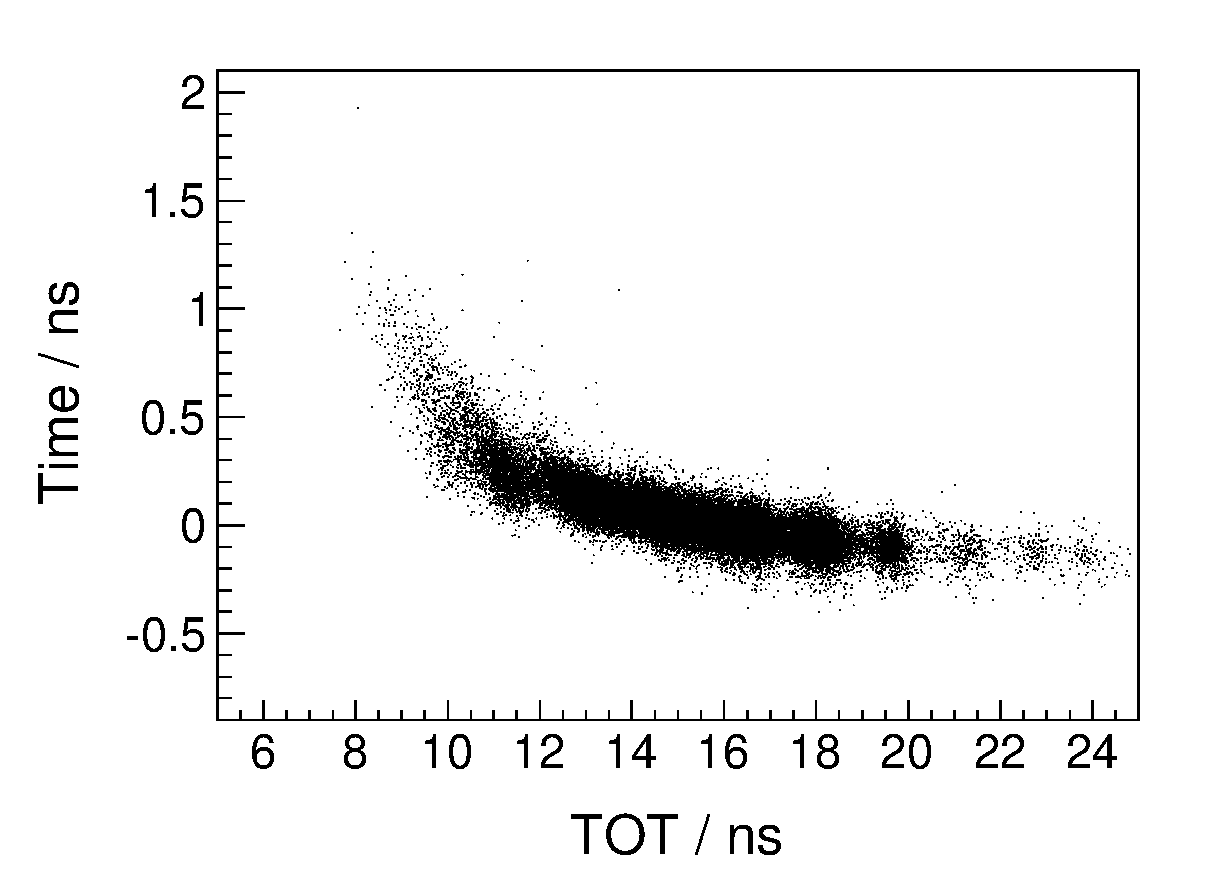
\includegraphics[width=0.9\textwidth]{chap3/afterCorZ-TOT.eps}
\caption{击中位置修正后时间对过阈时间的分布}
\label{fig:afterCorZ-TOT}
\end{figure}

基于此种分布,选用以下几种公式进行尝试,分别是:
\begin{align}
p_{0}+p_{1}/\sqrt{q}
\label{eq:1}\\
p_{0}+p_{1}/q
\label{eq:2}\\
p_{0}+p_{1}/q^{2}
\label{eq:3}\\
p_{0}+p_{1}/q^{3}
\label{eq:4}\\
p_{0}+p_{1}/\sqrt{q}+p_{2}/q
\label{eq:5}\\
p_{0}+p_{1}*q+p_{2}*q^{2}+p_{3}*q^3
\label{eq:6}    
\end{align}

比较公式~\ref{eq:1}~,~\ref{eq:2}~,~\ref{eq:3}~,~\ref{eq:4}~,~\ref{eq:5}~,~\ref{eq:6}~拟合的好坏,以及最终的时间分辨,分辨随~击中位置和过阈时间,MRPC模块的编号,读数条的编号等的分布,决定哪个是时间与过阈时间关系的主项。

\subsection{尝试各种公式}

\begin{figure}[!h]
\begin{minipage}{0.5\linewidth}
  \centerline{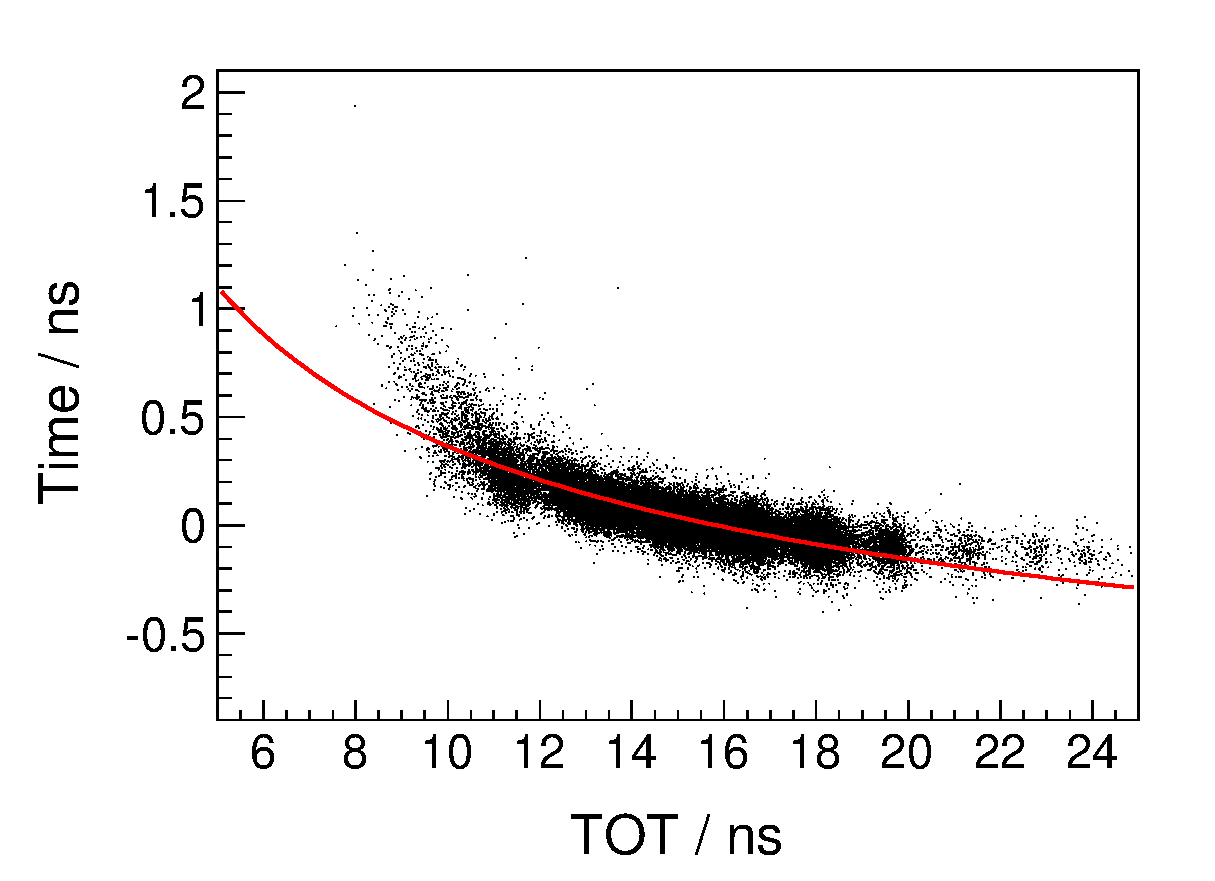
\includegraphics[width=0.9\textwidth]{chap3/half-order.eps}}
  \centerline{(a) 公式~\ref{eq:1}~的拟合}
  \centerline{\label{fig:half-order}}
\end{minipage}
\hfill
\begin{minipage}{0.5\linewidth}
  \centerline{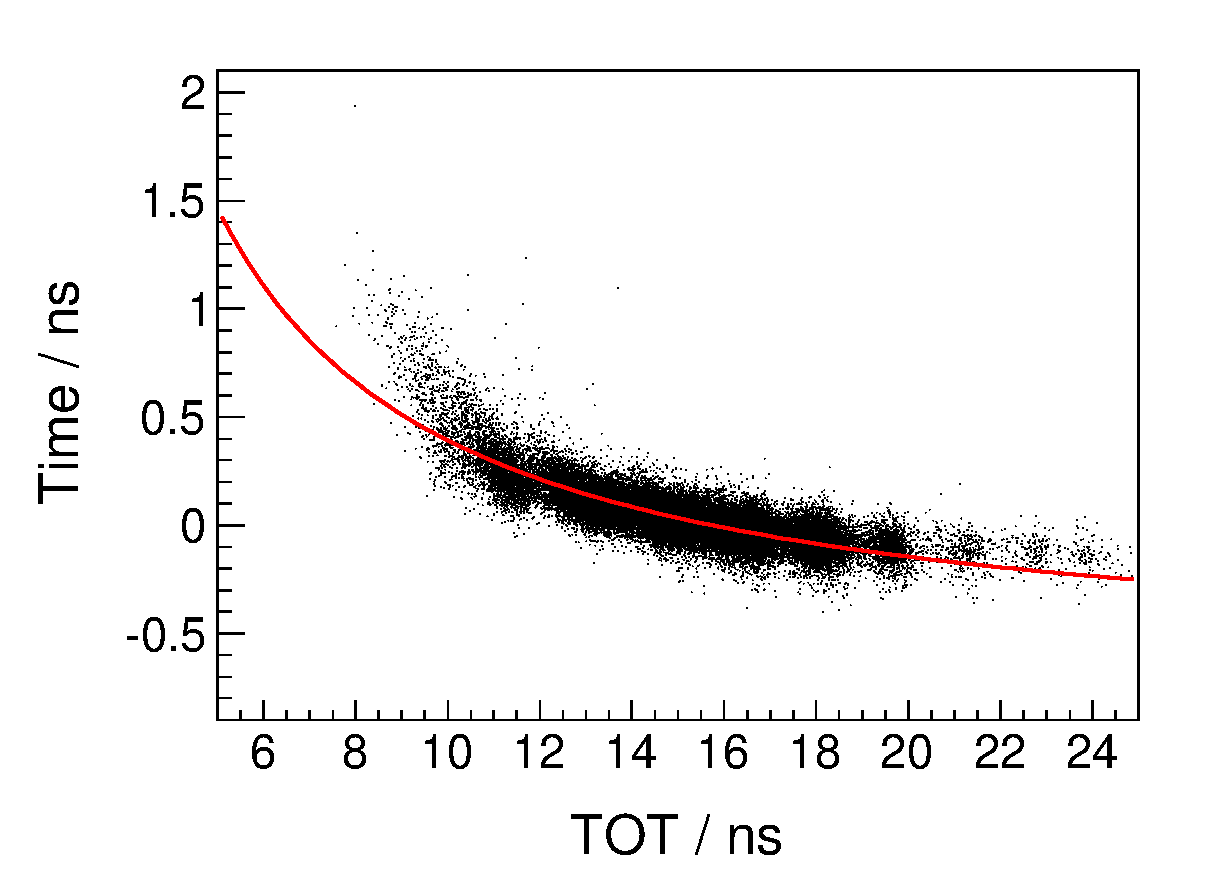
\includegraphics[width=0.9\textwidth]{chap3/1-order.eps}}
  \centerline{(b) 公式~\ref{eq:2}~的拟合}
  \centerline{\label{fig:1-order}}
\end{minipage}
\vfill
\begin{minipage}{0.5\linewidth}
  \centerline{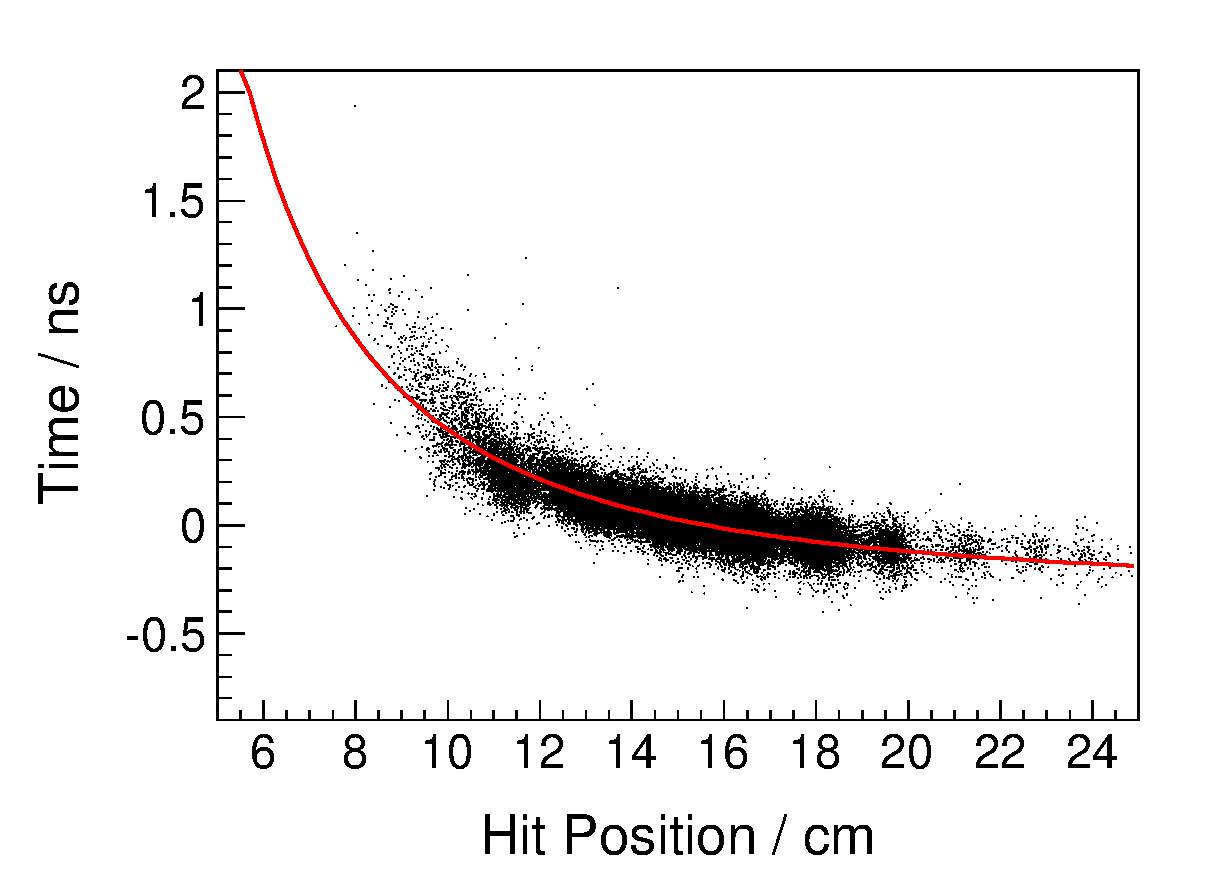
\includegraphics[width=0.9\textwidth]{chap3/2-order.eps}}
  \centerline{(c) 公式~\ref{eq:3}~的拟合}
  \centerline{\label{fig:2-order}}
\end{minipage}
\hfill
\begin{minipage}{0.5\linewidth}
  \centerline{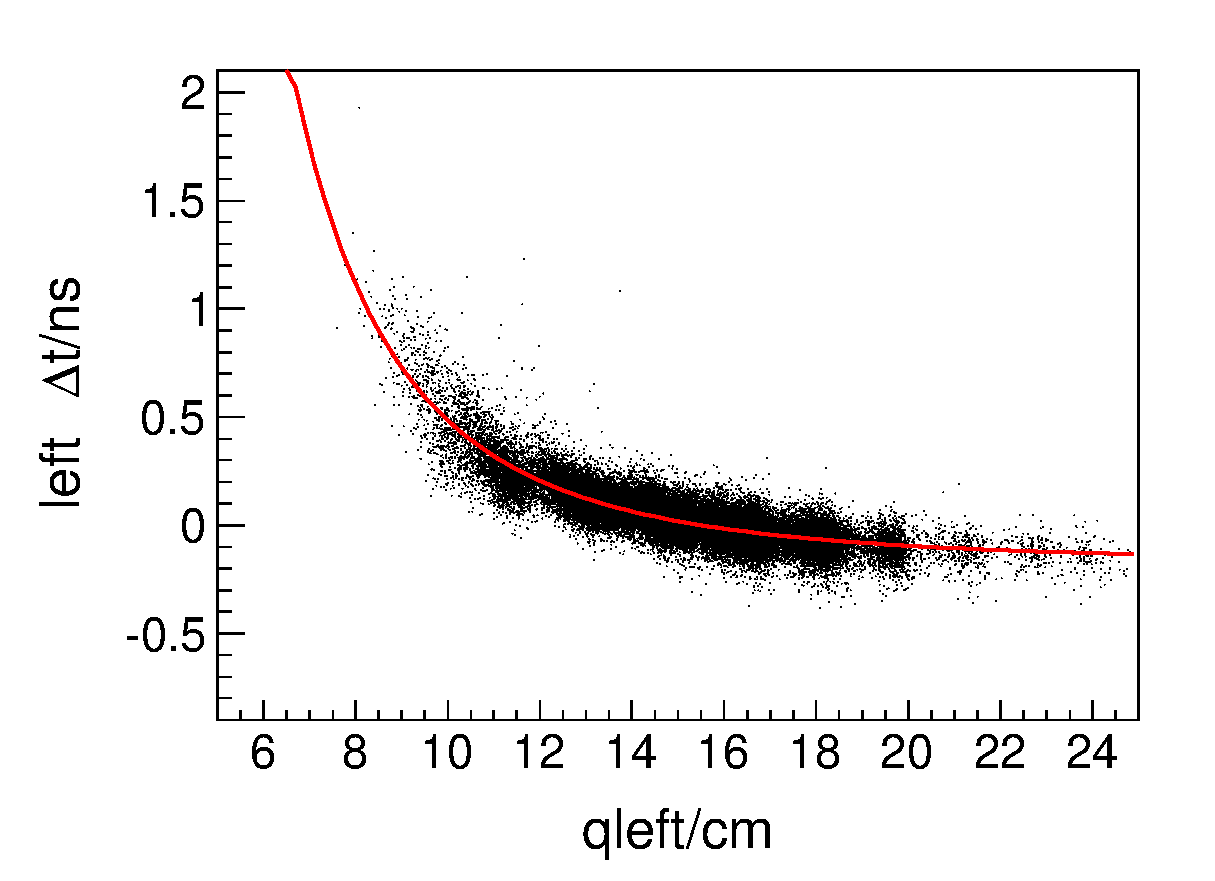
\includegraphics[width=0.9\textwidth]{chap3/3-order.eps}}
  \centerline{(d) 公式~\ref{eq:4}~的拟合}
  \centerline{\label{fig:3-order}}
\end{minipage}
\vfill
\begin{minipage}{0.5\linewidth}
  \centerline{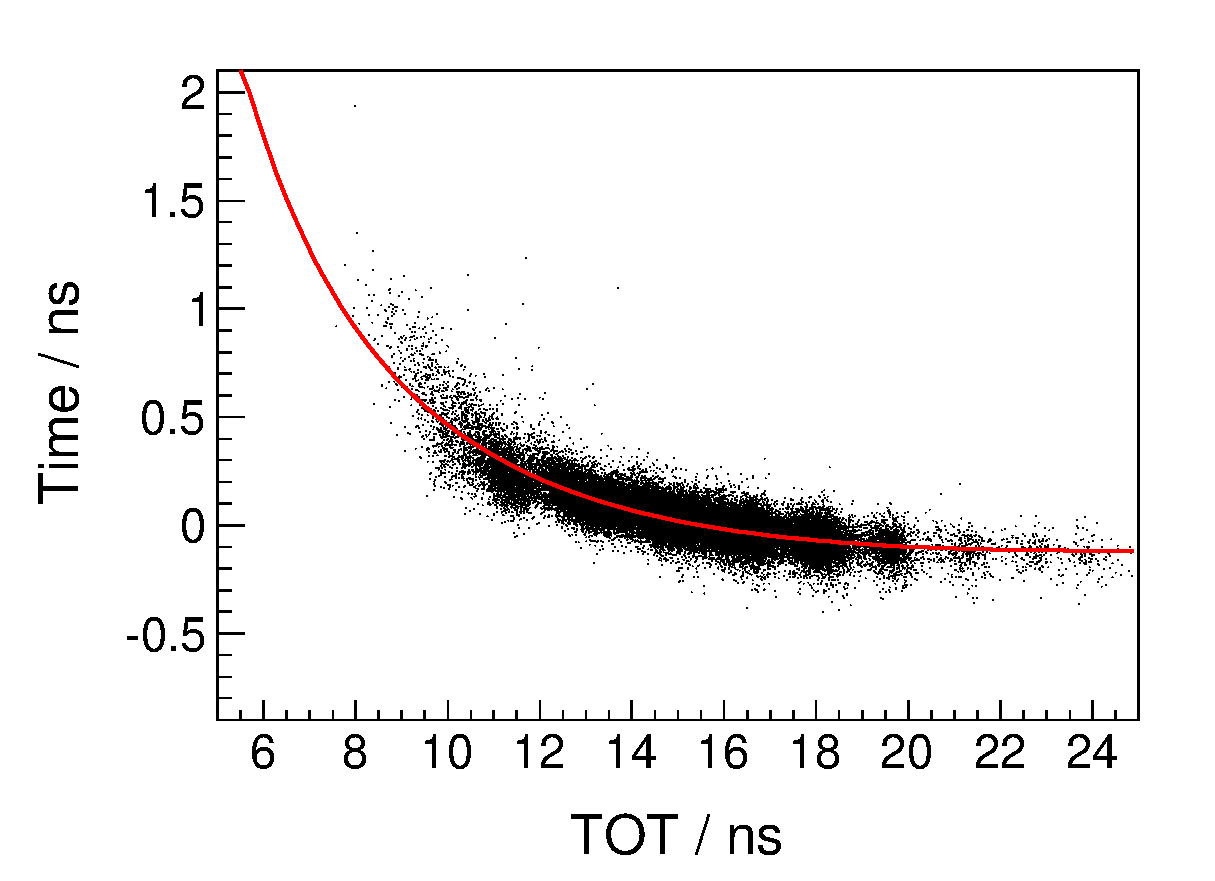
\includegraphics[width=0.9\textwidth]{chap3/half-1-order.eps}}
  \centerline{(e) 公式~\ref{eq:5}~的拟合}
  \centerline{\label{fig:half-1-order}}
\end{minipage}
\hfill
\begin{minipage}{0.5\linewidth}
  \centerline{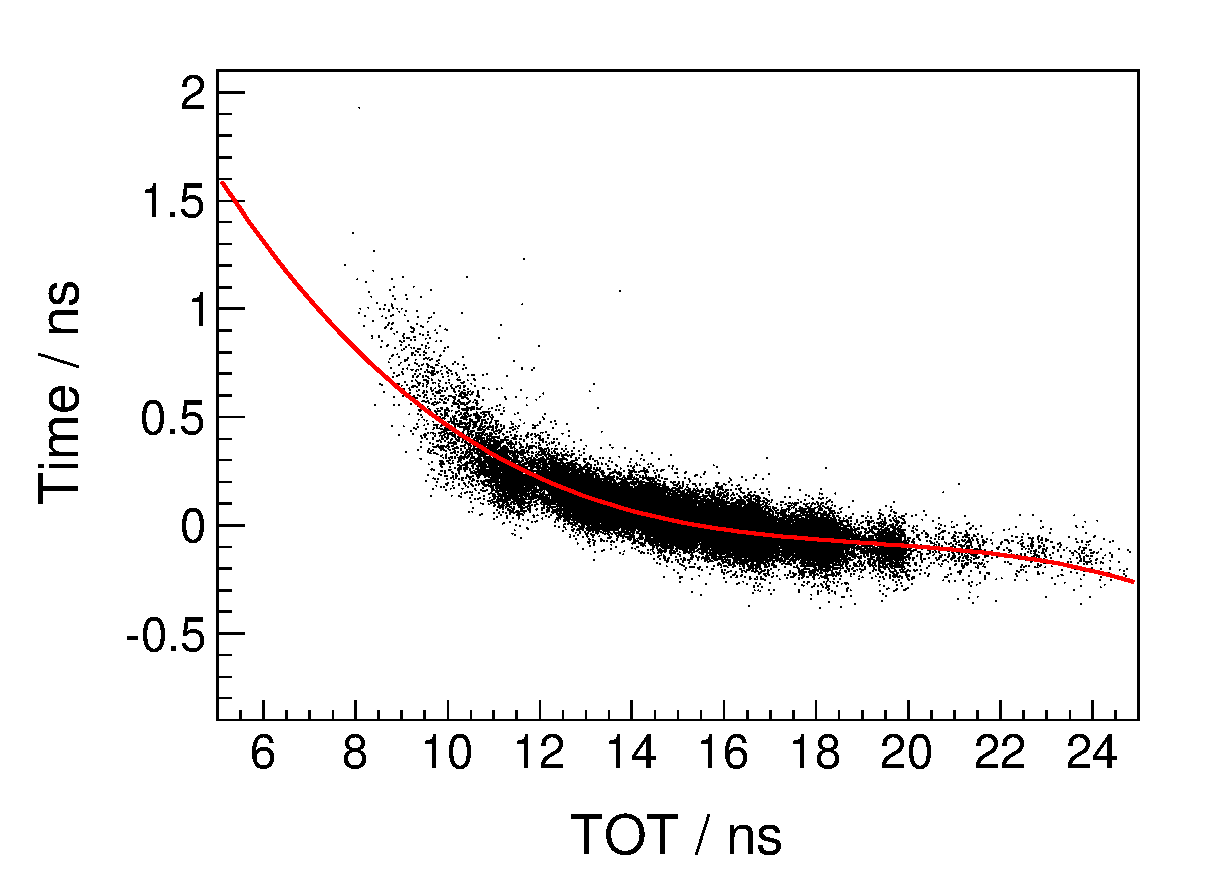
\includegraphics[width=0.9\textwidth]{chap3/pol3-order.eps}}
  \centerline{(f) 公式~\ref{eq:6}~的拟合}
  \centerline{\label{fig:pol3-order}}
\end{minipage}
\caption{几种公式对过阈时间的拟合}
\label{fig:single-formula}
\end{figure}
图~\ref{fig:single-formula}~是上述几种公式拟合的结果。
就这一条的拟合结果来看,公式~\ref{eq:3}~,~\ref{eq:4}~,~\ref{eq:5}~,~\ref{eq:6}~拟合的都不错。

表~\ref{tbl:resolution}~给出了这几种公式修正完成后得到的时间分辨。

\begin{table}[h]
    \centering
    \caption{\label{tbl:resolution} 上述公式修正后最终的时间分辨}
  \footnotesize
    \begin{tabular}{lc}
        \hline
        公式& 时间分辨(ps) \\
        \hline
        ${p_{0}+p_{1}/\sqrt{q}}$ & 65.6 \\
        ${p_{0}+p_{1}/q}$ & 65.1 \\
        ${p_{0}+p_{1}/q^{2}}$ & 63.9 \\
        ${p_{0}+p_{1}/q^{3}}$ & 63.9 \\
        ${p_{0}+p_{1}/\sqrt{q}+p_{2}/q}$ & 63.9 \\
        ${p_{0}+p_{1}*q+p_{2}*q^{2}+p_{3}*q^3}$ & 64.3 \\
        \hline
    \end{tabular}
\end{table}

\begin{figure}[!h]
\begin{minipage}[!h]{0.5\linewidth}
%\centering
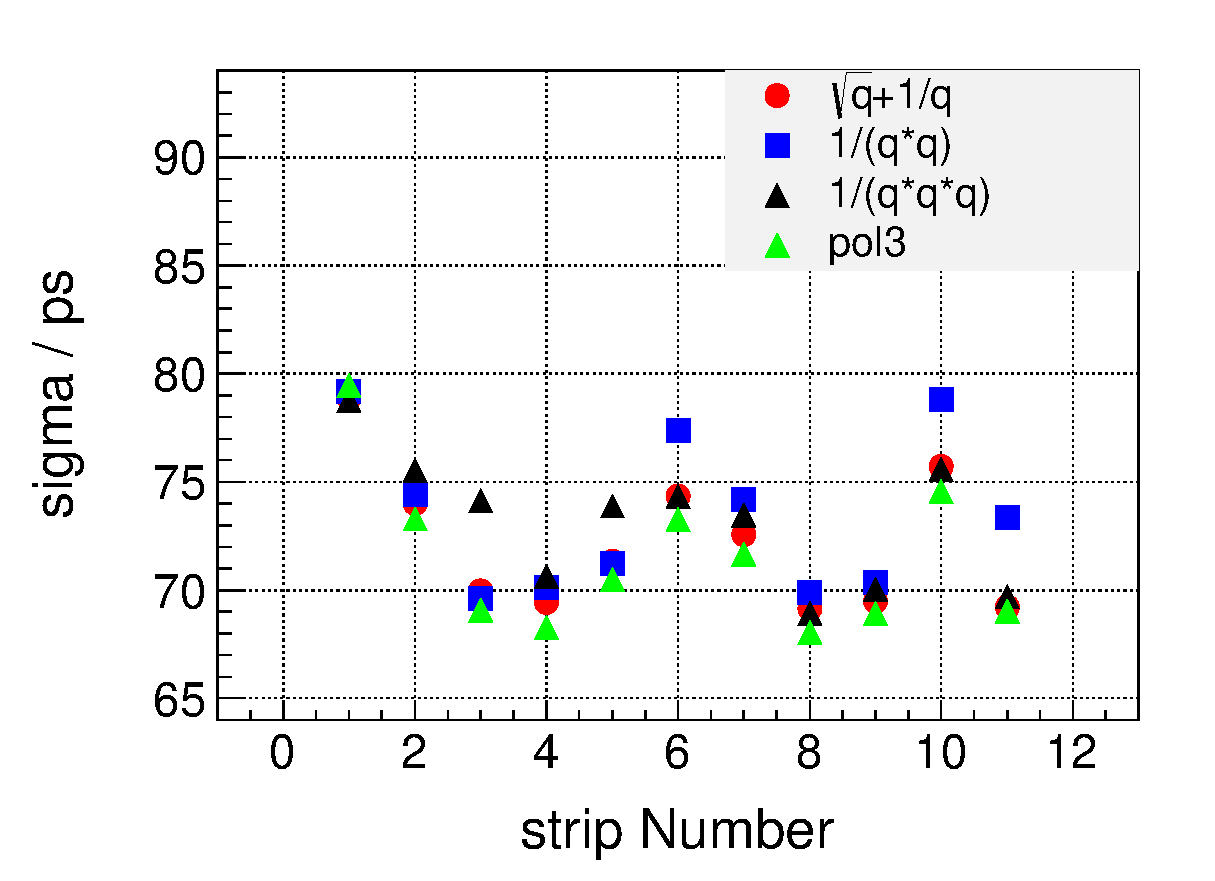
\includegraphics[width=0.9\textwidth]{chap3/single-module45.eps}
\subcaption{模块编号为45的几种公式时间分辨的比较}
\label{fig:single-module45}
\end{minipage}%
\hfill
\begin{minipage}[!h]{0.5\linewidth}
%\centering
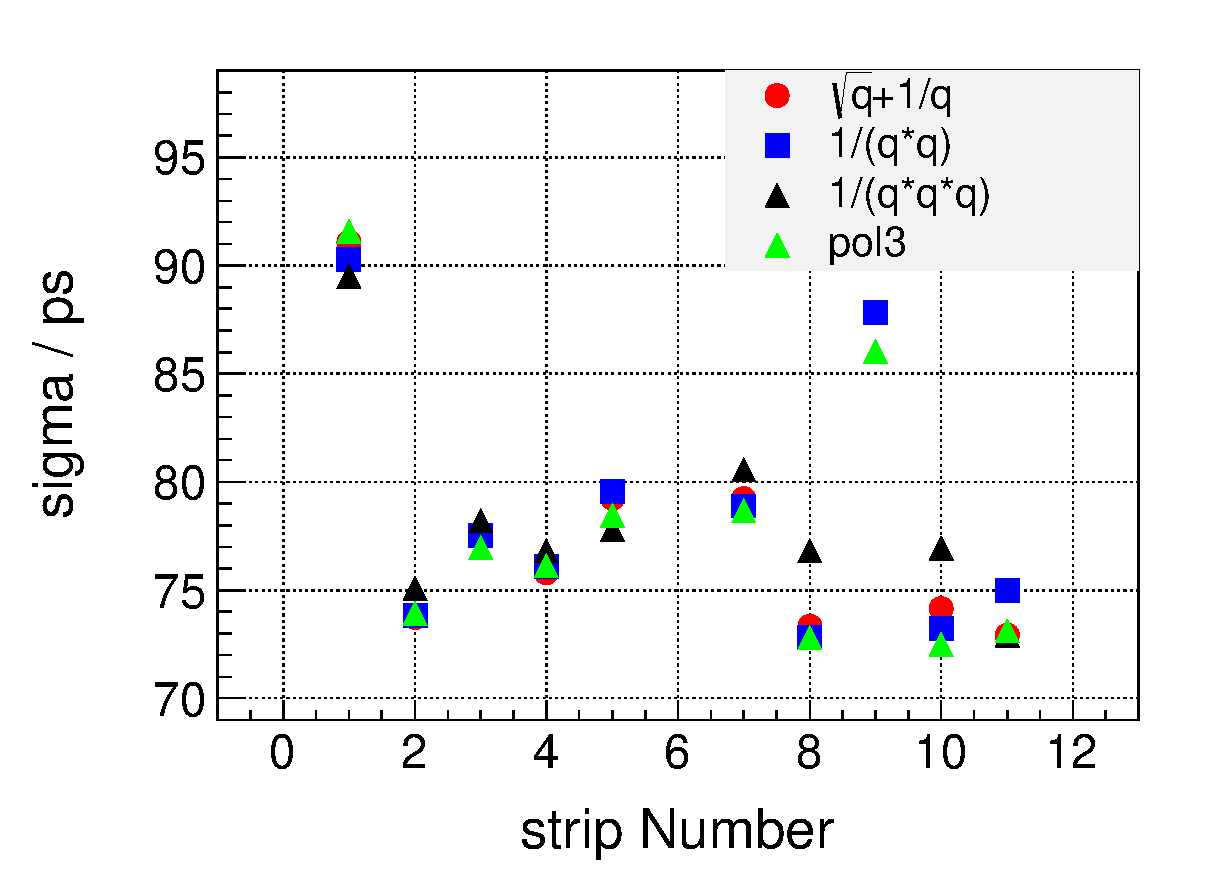
\includegraphics[width=0.9\textwidth]{chap3/single-module50.eps}
\subcaption{模块编号为50的几种公式时间分辨的比较}
\label{fig:single-module50}
\end{minipage}
\caption{几种公式修正得到的时间分辨的比较}
\end{figure}
在此研究的基础上随机选了两个模块,然后比较几种公式修正得到的时间分辨的。见图~\ref{fig:single-module45}~和图~\ref{fig:single-module50}~。可以看出,除了使用多项式外,公式${p_{0}+p_{1}/\sqrt{q}+p_{2}/q}$得到的时间分辨基本是最好的。对于多项式拟合而言,在~过阈时间比较大的一端拟合的并不足够好,并未真正的反映出时间随过阈时间的变化随着过阈时间的增大逐渐趋于平滑的这种趋势。

基于单条的拟合结果,以及比较多块的最终的时间分辨。
重点考虑选用公式~${p_{0}+p_{1}/\sqrt{q}+p_{2}/q}$~为刻度过阈时间的公式。在下一章关于双端公式的介绍部分会发现这个公式对于双端的拟合也是适用的。

\section{小结}

上章利用插值方法对~MRPC~的离线数据进行刻度,这章从另一个角度构造公式入手进行刻度。对于击中位置的修正,采用分~bin~,每个~bin~采用一个非对称的公式~Novosibirsk~拟合,最后对击中位置的修正采用一个三阶多项式拟合。而对于过阈时间的拟合,结合时间和过阈时间的分布关系,拟选取了几种可能能够描述这种分布关系的公式,经过比较几种公式,包括每个公式拟合的符合程度,以及随机选用两块比较这些公式的时间分辨。其中~${p_{0}+p_{1}/\sqrt{q}+p_{2}/q}$~是重点考虑的公式。









